%!TEX root=../../../main.tex

Using the base annotation model as a starting point, the targeted document
commenting feature can be implemented. In this scenario, the \textit{``where''}
field of the base model needs to encode both the document identifier and the
exact target of the annotation (e.g., the second page).

In the current version of Invenio, records can have one or more documents
associated, each of them with multiple versions. For example, during the CDS
paper review rounds, a single record will be used to upload multiple drafts of
the same document. Thus, annotations need to be attached to the correct version
of documents, in order to avoid displaying obsolete information. As the document
storage model is currently changing for the next version of Invenio, we have
chosen to implicitly attach annotations to the latest version of record
documents; nevertheless, this can be changed with minimal effort due to the
customisable nature of the JSON models.

\newpage

Regarding the document locations to which annotations can refer, after studying
over one thousand comments from CDS review rounds, we have chosen a total of
nine so-called \textit{``markers''} which can identify valid targets:
\begin{enumerate}
  \item Page (P)
  \item Figure (F)
  \item Line (L): this refers to the text line number which is sometimes used
                  in drafts (e.g., \LaTeX\ documents allow this when using the
                  \textit{``draft''} option for the document class). Optionally,
                  this could also be used in other configurations as, for
                  example, specifying a row in a table, or a relative line in a
                  paragraph.
  \item Equation (E)
  \item Table (T)
  \item Section (S): this could also refer to subsections as long as they
                     possess a proper identifier (e.g., Subsection 4.2 can be
                     marked using $S.4: S.2$).
  \item Paragraph (PP): this will likely refer to relative positions, such
                        as \textit{``the third paragraph on the second page''}.
  \item Reference (R): a bibliographic citation, could prove useful in a
                       scenario similar to the INSPIRE reference correction 
                       form presented in Section \ref{sec:motiv}.
  \item General (G): this allows specifying annotations which regard general
                     aspects, such as formatting issues (\textit{``the text is
                     not justified''}), or notes targeting currently nonexistent
                     elements (\textit{``a reference to the 2014 paper needs to
                     be added''}).
\end{enumerate}
The letters between parentheses above denote the special markup that can be
used by users for referring to the various document locations; for example,
\textit{``P.2: F.3a: equation system is not presumed''} is a valid annotation
on subfigure $3a$ on the second page. Markers can be combined to form
hierarchic structures with no depth restrictions; this should facilitate the
specification of precise, unambiguous locations.

This type of annotations can be inserted using the standard Invenio
commenting facilities, in two different manners:

\begin{itemize}
  \item Online, by using the form in Fig. \ref{fig:noteform}, which also
        provides a brief usage tutorial. Moreover, the aggregated view window in
        Fig. \ref{fig:noteview} can be used to point-and-click on the document
        previewer pane to add an annotation on the currently previewed page (the
        input form is pre-filled with the necessary markup).
  \item Offline, by using the described markup to edit the annotations while
        online access to the Invenio instance is not possible. Users can write
        their review, decorate it with the markup and add it later through the
        online form described above in order to be included with the rest of the
        comments. This is the reason for the markup being visible to the users
        and not implicit, directly encoded in the system by means of, for
        example, an interface similar to the one in Fig. \ref{fig:noteview}.
\end{itemize}

\begin{figure}[!ht]
  \centering
  \fbox{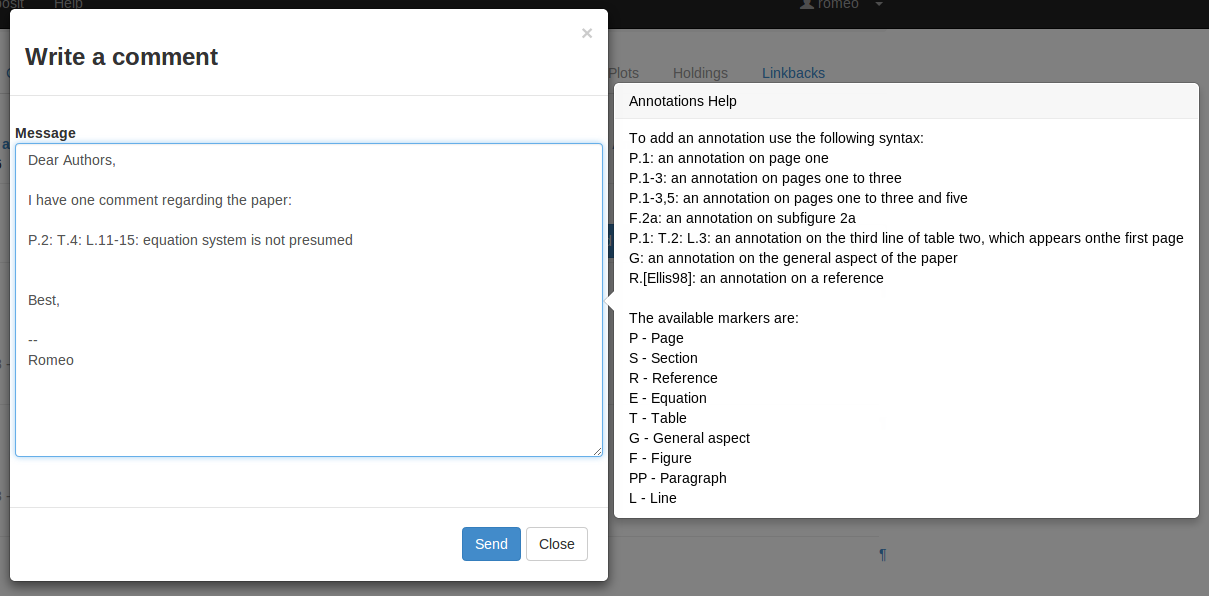
\includegraphics[scale=0.381]{static/img/commentform.png}}
  \caption[Invenio commenting form allowing annotation markup]
          {Invenio commenting form allowing annotation markup. To add remarks
           on any document element users can employ the markup described on the
           right-hand-side.}
  \label{fig:noteform}
\end{figure}

All the added record comments will be scanned and valid annotations will be
extracted by means of a simple regular expression mechanism. From a high level,
annotations are considered valid if complying with the following format:
\begin{verbatim}
  ^<MARKER 1>.<SPECIFIER 1>: [<MARKER 2>.<SPECIFIER 2>: ...
      [<MARKER N>.<SPECIFIER N>:]] <FREE TEXT>$
\end{verbatim}
Square brackets denote optional elements, and the \texttt{\^} and \texttt{\$}
symbols the beginning and end, respectively, of the text line; the line break
is inserted purely for formatting reasons. Specifiers are the actual locations
typed by the markers (e.g., page \textit{one}).

While the final regular expression used for extracting the annotations is quite
complex, it is composed of simple building blocks. For example, the section
marker is defined in a single line of code, as shown in Fig. \ref{lst:regex}.
Nevertheless, if the regular expression mechanism becomes too complex, or the
user requirements change by including new semantic validation rules (e.g., all
paragraphs need to be specified in relation to a section), the use of a
grammar could be considered.

\begin{figure}[!ht]
  \lstinputlisting[language=Python,
                   frame=tb,
                   basicstyle=\ttfamily,
                   captionpos=b,
                   numbers=none,
                   showspaces=false,
                   showstringspaces=false,
                   showtabs=false,
                   stepnumber=2,
                   numbersep=4pt]
    {static/lst/regex.py}
    \caption[Regular expression marker definition for sections]
            {Regular expression marker definition for sections. The regular
             expression is defined as the marker ($S$), followed by a full stop,
             followed by list of alpha-numeric characters of length equal or
             greater than $1$ (the global definition of $LOCATION$ is currently
             used for almost all markers).}
    \label{lst:regex}
\end{figure}

\newpage

Extracted annotations will be saved in a JSON document complying with the
JSONAlchemy template, in the MongoDB database. It is worth noting that these
annotations are stored along with the ones described Subsection \ref{sec:gra}
in the same \textit{collection} (equivalent of a SQL table); this is made
possible by the fact that the database accepts dynamic schemas and not rigid,
pre-defined ones.

To summarise, the model for targeted document annotations is similar to the
base one presented in Section \ref{sec:gra}, except for the \textit{``where''}
field which is composed of the record identifier and document marker(s), and a
new field containing the identifier of the comment in which the annotation
originated (used for providing context to end-users). A remark here is that in
order to use more standard IRI locators for the target, as in the base model, a
scheme that allows navigating to a preview of the specified document location
could be used.  For example, \texttt{/record/1/annotations/page1-paragraph2/}
could be employed to open a previewer highlighting the specified text region.
This is currently implemented only for page numbers, due to technical
limitations of the document previewer solution.

For completeness, the workflow of document annotations is included in Fig.
\ref{fig:docanno}.

\begin{figure}[!ht]
  \centering
  \fbox{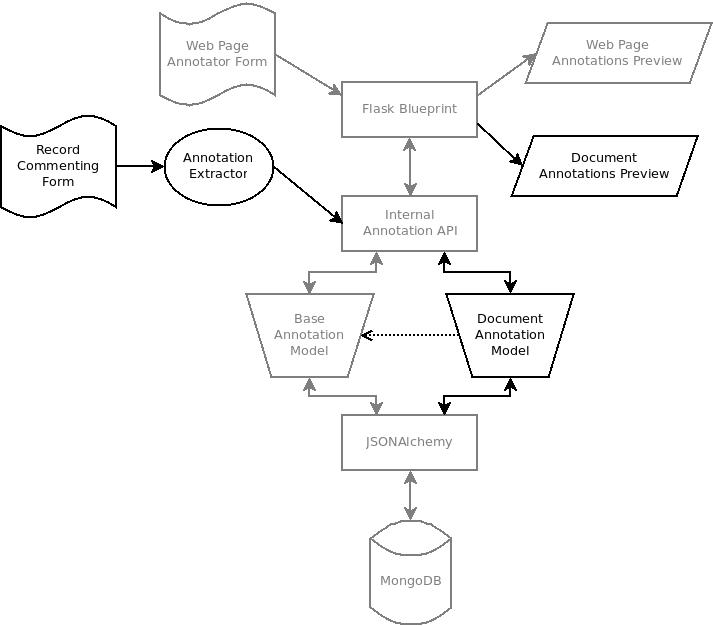
\includegraphics[scale=0.6]{static/dia/doc_anno.jpeg}}
  \caption[Document annotation workflow]
          {Document annotation workflow; the base annotation model is extended
           to allow adding notes on specific document locations (e.g., page,
           figure, equation). Annotations are extracted from basic Invenio
           comments, by identifying the special markup that can be employed by
           users in order to refer to locations.}
  \label{fig:docanno}
\end{figure}

\FloatBarrier

Finally, annotations can be previewed in a manner similar to the one presented
in Fig. \ref{fig:noteview}. The current version proposes a two-column window,
with one column dedicated to previewing the concerned document (currently the
supported format is PDF), and the other to displaying annotations. Coming
back to the CDS review process use-case, the annotation display has been
designed in a manner addressing two issues:
\begin{enumerate}
  \item Separate targeted annotation from free-text comments: even if a comment
        includes both markup decorated and non-structured content, the
        aggregated view will display only the notes targeting a specifying
        aspect. Considering the following comment:
        \begin{verbatim}
          Dear authors,

          This is a very good paper, but I have the following remark:
          P.2: F.3a: equation system is not presumed 
        \end{verbatim}
        only the remark on subfigure $3a$ on the second page will be displayed.
        The complete comments can still be accessed in the standard Invenio
        manner.
  \item Aggregate remarks by location, to allow the authors in charge of
        amending the paper to systematically follow them. As can be observed in
        Fig. \ref{fig:noteview}, annotations are first grouped by page and then
        hierarchically, in a top--down manner, from the most general marker to
        the most particular one.
\end{enumerate}

\begin{figure}[!ht]
  \centering
  \fbox{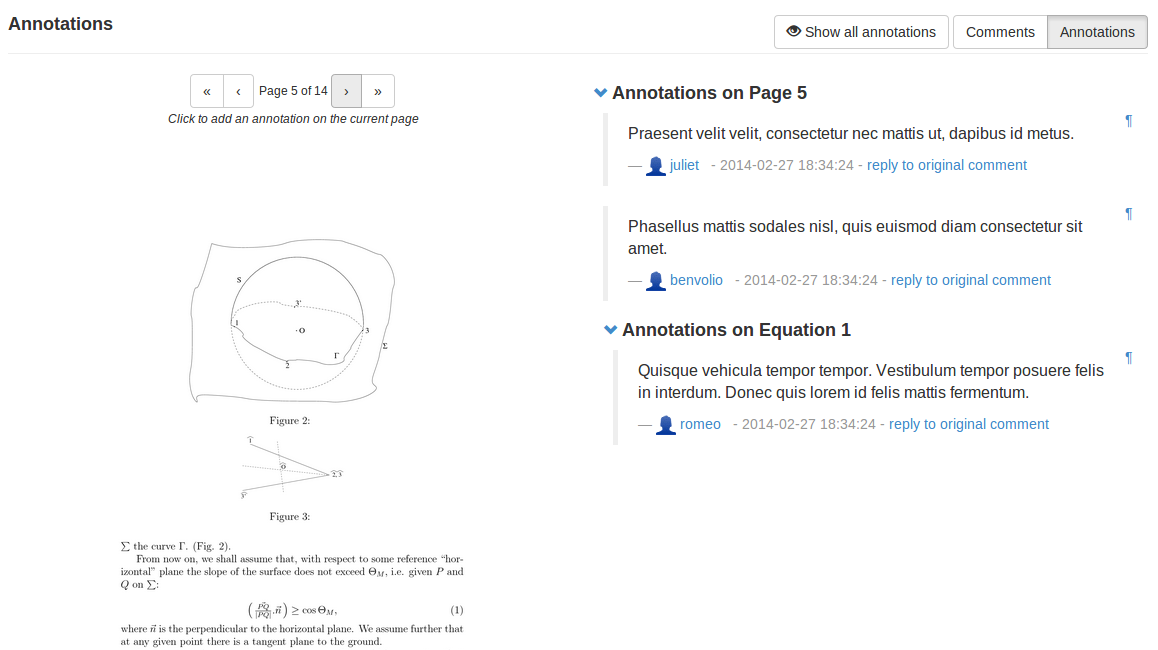
\includegraphics[scale=0.398]{static/img/noteview.png}}
  \caption[Document annotation previewer]
          {Document annotation previewer. A PDF document preview is included on
           the left-hand-side, while the annotations on the currently displayed
           page are presented on the right-hand-side; annotations are
           furthermore aggregated, depending on their sub-markers (e.g.,
           Equation 1). Clicking on the previewer pane allows adding a new
           annotation targeting the displayed page.}
  \label{fig:noteview}
\end{figure}
